\section{INTRODUCTION}
\label{S:intro}

\textcolor[rgb]{0,0,1}{Control-oriented predictive models of an energy system's dynamics and energy consumption, are needed for understanding and improving the overall energy efficiency and operating costs of a building.
With a reasonably accurate forecast of future weather and building operating conditions, dynamical models can be used to predict the energy needs of the building over a prediction horizon, as is the case with Model Predictive Control (MPC) \cite{Sturzenegger2016}.
However, a major challenge with MPC is in accurately modeling the dynamics of the underlying physical system.
The task is much more complicated and time consuming in the case of a large building and often times, it can be even more complex and involved than the controller design itself.
After several years of work on using first principles based models for peak power reduction, energy optimization and thermal comfort for buildings, multiple authors~\cite{Sturzenegger2016, vzavcekova2014} have concluded that the biggest hurdle to mass adoption of intelligent building control is the cost, time and effort required to capture accurate dynamical models of the buildings.
The user expertise, time, and associated sensor costs required to develop a model of a single building is very high. Thus, the payback period for the upfront hardware and software installation is expected to be too high, making MPC an uneconomical choice for energy management.}

\textcolor[rgb]{0,0,1}{Why is physics-based modeling hard for complex systems like buildings or what are the reasons of such modeling complexities?}
\begin{enumerate}
	\item \textcolor[rgb]{0,0,1}{\textbf{Model capture} - a building modeling domain expert typically uses a software tool to create the geometry of a building from the building design and equipment layout plans, add detailed information about material properties, about equipment and operational schedules. There is always a gap between the modeled and the real building and the domain expert must then manually tune the model to match the measured data from the building~\cite{New2012}. 
	Moreover, the modeling process also varies from building to building with the construction and types of installed equipment.
	Another major downside with physics-based modeling is that enough data is not easily available and guesses for parameter values have to be made, which also requires expert know-how.
	\item \textbf{Change in model properties over time} - even if the model is identified once via an expensive route as in \cite{Sturzenegger2016}, as the model changes with time, the system identification must be repeated to update the model. Thus, model adaptability or adaptive control is desirable for such systems.
	\item \textbf{Model heterogeneity} further prohibits the use of model-based control. For example, unlike the automobile or the aircraft industry, each building is designed and used in a different way. Therefore, this modeling process must be repeated for every new building. }
\end{enumerate}

\textcolor[rgb]{0,0,1}{Due to aforementioned reasons, the control strategies in such systems are often limited to fixed, sometimes ad-hoc, rules that are based on best practices. 
The alternative is to use black-box, or completely data-driven modeling approaches, to obtain a realization of the system's input-output behavior. 
The primary advantage of using data-driven methods is that it has the potential to eliminate the time and effort required to build white and grey box building models. 
Listening to real-time data, from existing systems and interfaces, is far cheaper than unleashing hoards of on-site engineers to physically measure and model the building. Improved building technology and better sensing is fundamentally redefining the opportunities around smart buildings. 
Unprecedented amounts of data from millions of smart meters and thermostats installed in recent years has opened the door for systems engineers and data scientists to analyze and use the insights that data can provide, about the dynamics and power consumption patterns of these systems. }

\textcolor[rgb]{0,0,1}{The key question now is: can we employ data-driven techniques to reduce the cost of modeling, and still exploit the benefits that MPC has to offer?
We therefore look for automatic data-driven approaches to control, that are also adaptive, scalable and interpretable.
We solve this problem by bridging Machine Learning and Predictive Control. In particular, in this paper, we present a method based on Random Forests which uses historical data for receding horizon control.}

\textcolor[rgb]{0,0,1}{
Next, we present an example to illustrate how data-driven modeling reduces the cost of modeling buildings. 
}

%\paragraph{Example} \textcolor[rgb]{0.00,0.00,1.00}{As a first} example of such modeling complexity, consider the grey-box approach in \cite{Braun2002}. The scope of such approach is to predict the heat transfer rate to the air within the building. In particular, the authors addressed a single zone modeling problem using an equivalent $RC$ model. To this end, five different types of structures are considered in the example: external walls, ceiling/roof, floor, internal walls and windows. Each of these elements are represented using $3$ resistances, $2$ capacitances and $2$ temperatures, except for the windows that are represented only with resistances since they have a negligible energy storage. A model consisting of $8$ states and $9$ inputs, including disturbances such as solar radiation and others, with the instantaneous heat gain to the building air from all surfaces as output, is created for the zone. To have a complete LTI model, $9$ parameters are needed to be estimated via a non-trivial training process, using a collection of information associated with a physical description of the building (see \cite{Braun2002} for more details). Extending this result, for the building we consider in Section \ref{S:realCaseStudy} with $10$ different zones, we would need to consider a model with approximately $80$ states and $90$ parameters to be estimated.

\subsection{Example for comparison of modeling complexity: physics-based vs data-driven}
\textcolor[rgb]{0,0,1}{In this section, we provide a detailed example that describes the difference in terms of complexity when we model a building using physical laws and machine learning.
We show that the data-driven modeling eliminates several drawbacks that occur using physics-based models such as the need to have very good knowledge of the building structure and the material properties, time required to build a model, and limited availability of sensor measurements.}

\textcolor[rgb]{0,0,1}{The building under consideration is taken from \cite{Sturzenegger2016}. It is located in Allschwil, Switzerland. It has 6 floors of which only the second floor is modeled, and is assumed to represent all other floors. The total air conditioned floor area is $6000\ \mathrm{m^2}$ ca.}

\subsubsection{Physics-based modeling}
\label{SSS:physics-based}
\textcolor[rgb]{0,0,1}{We describe the physics-based approach based on an RC network outlined in \cite{Sturzenegger2016}.
The building is modeled as a bilinear system constructed from physical principles.
The modeling process consists of three steps:
\begin{enumerate}
	\item Building geometry and construction data are used together with first-principles to derive the following linear model for the building's thermal dynamics:
		\begin{equation}\label{E:RCZoneEq}
			\dot x(t) = A_x x(t) + B_q q(t).
		\end{equation}
		This model describes the behavior of the zone, wall, floor and ceiling temperatures.
		Walls, floors and ceilings are considered as divided into layers with different features. Therefore, each zone was described with an RC network model (see Figure 3-10 in \cite{SturzeneggerTR}), where the capacitances represent the states of the layers and the resistances represent the thermal resistance of the layers.
%		\begin{figure}[t]
%			\begin{center}
%				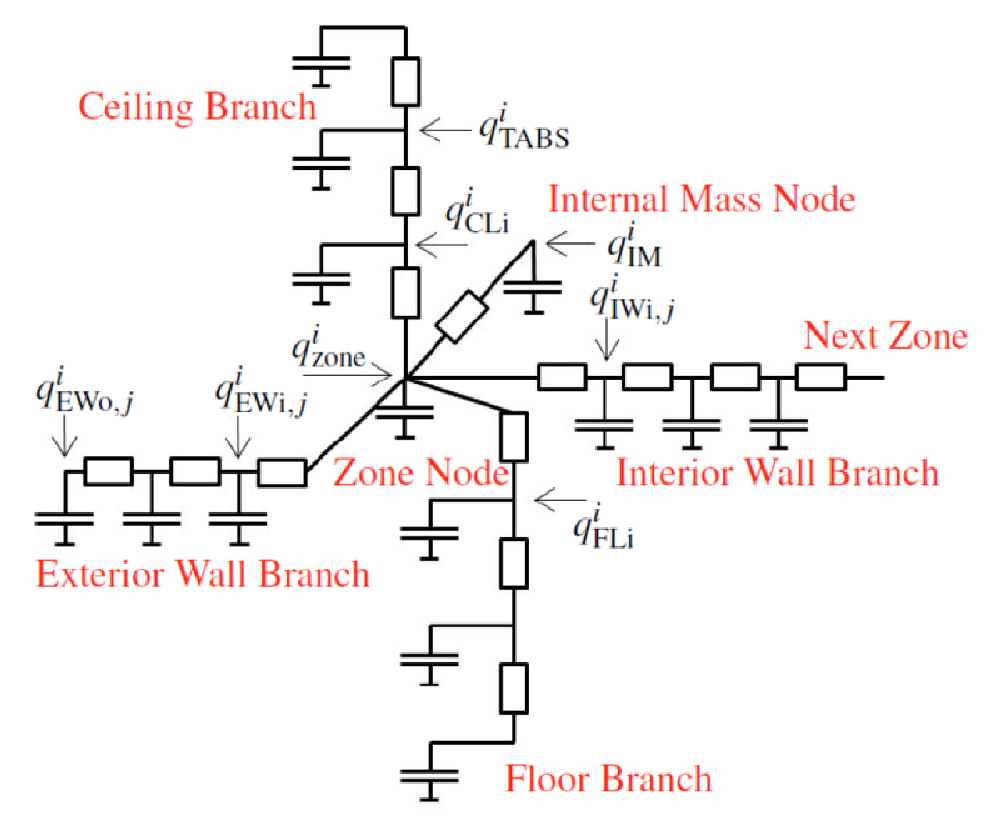
\includegraphics[width=0.6\textwidth]{figures/RC_net.eps}
%				\caption{RC model of a zone. $q$ represents the external heat fluxes}\label{F:RCnet}
%			\end{center}
%		\end{figure}
		The heat exchange between two adjacent layers, i.e. layer ``a" and layer ``b", is modeled to be proportional to the temperature difference of the two layers and the corresponding thermal resistance $R$ given by
		\begin{equation}\label{E:RCHeatExchange}
			\begin{aligned}
				&C_a\dot x_a = \frac{x_b(t) - x_a(t)}{R},\\
				&C_b\dot x_b =  \frac{x_a(t) - x_b(t)}{R},
			\end{aligned}
		\end{equation}
		where $C_a$ and $C_b$ are the heat capacitances of the layers. This is done for each layer of each zone, obtaining the compact representation given in \eqref{E:RCZoneEq}. The thermal parameters are derived from zones geometry and material properties.
	\item External heat fluxes, modeled as a bilinear model, affect the building directly as well as indirectly through zones:
		\begin{equation}\label{E:RCfluxes}
			q(t) = A_q x(t) + B_{q,u}u(t) + B_{q,d}d(t) + \sum_{i=1}^{n_u}{[\left(B_{q,du,i}d(t) + D_{q,xu,i}x(t)\right)u_i(t)]},
		\end{equation}
		where $u$ are the inputs and $d$ the disturbances of the system.
%		Equation \eqref{E:RCfluxes} comes from a series of 20 equations analyzed in Section 3.3.1.3 of the Technical Report \cite{SturzeneggerTR}, that we do not report here for the sake of simplicity. 
Equation \eqref{E:RCfluxes} for the heat flux is obtained by modeling
	\begin{enumerate}
		\item heat exchange associated with the building hull (except for windows), both conductive and radiative part,
		\item  heat flux to each thermally activated building system (TABS), i.e. pipes buried in the concrete slabs of the floors carrying hot/cold water,
		\item heat flux through the windows in three different parts: radiation due to elements directly in contact with the zone air, conduction through the window, and absorption of the solar radiation through the window,
		\item convection due to internal gains due to occupants, appliances and lighting, and
		\item the effects of the AHU.
	\end{enumerate}
	\item The resulting system \eqref{E:RCZoneEq} is discretized with a sampling time of $15\ \mathrm{min}$.
	This model has approximately 300 states that include temperature of the zones, walls and floors on the second floor.
	The outputs of the system are the zone temperatures.
	Since the performance of the state estimation, that is needed to compute the optimal control inputs using MPC depends on the number of states, an approximated model with fewer states is needed.
	To this aim, different averaged temperatures of the building facades (North, South, West, East) and the zones are considered, obtaining an approximated model with 35 states.
	This  approximate model is then considered ``suitable for MPC" (see Section 3.3.1.4 in \cite{SturzeneggerTR}). 
\end{enumerate}}
	
\textcolor[rgb]{0,0,1}{In summary, the approximate model has the following state, input and disturbance variables:
	\begin{itemize}
		\item 5 outputs: averaged room temperature for each group of zones (North, South, West, East, Center). The rooms are equipped with temperature sensors.
		\item 18 inputs: TABS heating heat flux, TABS cooling heat flux, averaged transmitted solar heat flux for each group of zones (North, South, West, East) that is estimated using blinds position measurements, air massflow through the energy recovering mode, air massflow bypassing the energy recovering mode, air massflow through the air cooler, AHU heat coil heat flux, lighting power for the offices for each group of zones (North, South, West, East), and radiator heat flux in the corner offices (North, South, West, East).
		\item 7 disturbances: internal gains in the offices and internal gains in non-office zones, which are predicted using a standard schedule, ambient temperature and solar radiation on facade (North, South, West, East) whose values were obtained through Kalman filtering using measurements from the weather station placed on the roof of the building. This filtering is needed to take into account the shadowing of the neighboring buildings.
	\end{itemize}
An EnergyPlus model is built for this system, and model parameters of matrices $A_x$, $B_q$, $A_q$, $B_{q,u}$, $B_{q,d}$, $B_{q,du,i}$, $D_{q,xu,i}$ in Equations \eqref{E:RCZoneEq} and \eqref{E:RCHeatExchange} are derived using geometry and materials data from the EnergyPlus model.
This was a choice of the authors; real geometry and materials data can also be used to estimate the model parameters, if necessary data are available. 
For this particular building, 24 parameters are estimated/taken form a datasheet/computed for the considered zone model.
Although some of the parameters are in common between different zones, the others are found independently for each zone.
To simplify, the parameters of all the other floors are assumed to be identical which is not true in reality.
To derive the EnergyPlus model using the available measurements and to use the same control implemented in the building, the EnergyPlus model is coupled with MATLAB using BCVTB \cite{Wetter2015}.
}
%To identify the model a total of 294 MATLAB signals were sent to the EnergyPlus model and a total of 1081 EnergyPlus signals were sent back to Matlab.

\textcolor[rgb]{0,0,1}{The physics-based approach, although detailed and accurate (in some cases), is cost and time prohibitive. The long and complex modeling procedure that is unique to every building poses practical challenges in applying MPC to large scale buildings.}

\subsubsection{Data-driven modeling}
\textcolor[rgb]{0,0,1}{The data-driven approach we propose, on the other hand, ignores the physical details of the building operation. Instead, we use machine learning to learn black-box models where our objective is to find the hyperparameters (for a given structure like Random Forests) of a model that best explains the input-output relationship.}

\textcolor[rgb]{0,0,1}{The goal with the data-driven modeling is to learn a function map
\begin{equation}
\label{E:MLexample}
y(t) = f(u(t),\dots,u(t-\delta_u), d(t),\dots, d(t-\delta_d)),
\end{equation}
where \(y\) represents the outputs, \(u\) the inputs and \(d\) the disturbances as defined earlier, and \(\delta\) is a lag variable.}

\textcolor[rgb]{0,0,1}{The data-driven modeling in the case of buildings has several advantages over the physical counterpart.}
\begin{enumerate}
	
	\item \textcolor[rgb]{0,0,1}{\textbf{Domain expertise:} 
	This procedure (\textcolor[rgb]{1,0,0}{NOT CLEAR IF EXPLAINED IN ONLY 2 LINES BEFORE}) eliminates the need of a building expert, simplifies the modeling complexities (\textcolor[rgb]{1,0,0}{HOW?}) described in Section \ref{SSS:physics-based} which ultimately reduces the cost of modeling a building. Further, for a new building, given the historical data from the building, the same process can be repeated to identify a control-oriented model for MPC.}
	
	\item \textcolor[rgb]{0,0,1}{\textbf{Sensor cost:}
	Due to large number of states and variables in the physical modeling, a lot of measurements are needed to use the model to predict the system's behavior \textcolor[rgb]{1,0,0}{IF USING A MODEL-BASED APPROACH}.
	This can be expensive due to necessary new sensor installations.
	Moreover, when some measurements are not directly available from the sensors, observers are needed for state estimations.
	However, observability problems can limit the construction of such observers \cite{Dorf2011MCS}. 
	On the other hand, data-driven modeling obviates the need to model the state of the walls and floor layers\textcolor[rgb]{1,0,0}{AND OTHER STATES DIFFICULT TO MEASURE} so we do not have as many states.\textcolor[rgb]{1,0,0}{EXPLAIN THAT THE MACHINE LEARNING ALGORITHM IS ABLE TO COMPENSATE MISSING VARIABLES}
	It relies only on direct measurements from the sensors such as thermostats and multimeters reducing the need for new installations and hence the cost of modeling.
	Further, when some of the states are not directly measurable, often adding proxy \textcolor[rgb]{1,0,0}{I.E. ??}variables suffices. 
	For example, if we do not have the measurement of the energy produced by a photovoltaic panel, the weather conditions will account for it.}
	
	\item \textcolor[rgb]{0,0,1}{\textbf{Linearity assumption:}
	If \(y\) in Equation \eqref{E:MLexample} is the average room temperature for one of the zones, a nonlinear function \(f\) is more appropriate, for example \(f\) may belong to the class of Neural Networks or Random Forests. 
	During physical modeling in \eqref{E:RCHeatExchange}, in order to keep the model simple, the heat exchange between layers is modeled with a linear behavior. 
	Hence all the nonlinearities were neglected.
	In the case of heat flux in \eqref{E:RCfluxes}, again, a linear model is not good enough to provide a good approximation. For this reason a bilinear model was considered.
	However, more complex nonlinearities have been neglected due to the already high complexity of the model \cite{Sturzenegger2016}. 
	In data-driven modeling, we can relax these linearity assumptions as nonlinear functions can be learned rather efficiently and accurately.\textcolor[rgb]{1,0,0}{IT IS NOT CLEAR THAT THE DD ALGORITHM TAKE CARE OF IT CREATING ITS INTERNAL STRUCTURE}}
	
	\item \textcolor[rgb]{0,0,1}{\textbf{Other assumptions:} 
	Due to the high modeling complexity, physical modeling neglects different geometries and different materials of the floors assuming they are the same for each floor which is never true in reality.
	In many cases, the details of construction layout and equipments are not even available so many parameters have to be guessed.
	Data-driven modeling depends on the sensor data directly. 
	Hence, such assumptions never arise.}
	
\end{enumerate}

\textcolor[rgb]{0,0,1}{To summarize, the data-driven modeling simplifies the modeling of buildings to a large extent, reduces the overall cost and time investment while avoiding the linear model assumptions that we make in standard physical modeling procedure. Unlike physical modeling, the parameters of the model (or hyperparamters) are automatically determined by the learning algorithm, the best settings determined by cross validation.}

\textcolor[rgb]{0,0,1}{However, the challenge lies in using such models for optimal predictive control, which is exactly the focus of this paper.
We demonstrate how the training algorithm for Random Forests can be modified to develop control oriented models that are suitable in the MPC framework.}

\textcolor[rgb]{0,0,1}{
\subsection{Related work}
A vast literature exists in building energy applications that deals with Demand Response, peak power reduction, energy saving, thermal comfort, and related topics.
All these approaches can be classified based on two characteristics:
\begin{enumerate}
	\item the type of system model:
		\begin{itemize}
			\item model-based, that we consider both "white-box" and "grey-box" approaches: \cite{Shakouri2017SCS,Li2014EB,Yoon2014EB,Li2016AE,Harb2016EB,Salakij2016EB,Li2016E,Li2016EB,Hou2013,Cecconi2017EB};
			\item data-based, that is the "black-box" approach, mainly done using Neural Networks: \cite{Safa2017SCS,Neto2008EB,Magnier2010BE,Candanedo2017EB,Ascione2017E,Cecconi2017EB,Li2016AE};
			\item simulation tool-based, such as EnergyPlus \cite{energyPlus} and TRNSYS \cite{trnsys2000}: \cite{Yin2016EB,Christantoni2016EB};
		\end{itemize}
	\item the purpose these models are created for:
		\begin{itemize}
			\item only model creation and identification: \cite{Safa2017SCS,Neto2008EB,Magnier2010BE,Li2014EB,Li2016AE,Harb2016EB,Li2016EB,Candanedo2017EB,Cecconi2017EB,Ascione2017E};
			\item model identification and control (typically Predictive Control): \cite{Shakouri2017SCS,Yoon2014EB,Yin2016EB,Salakij2016EB,Li2016E,Hu2017AE}.
		\end{itemize}
\end{enumerate}
These papers are summarizes in Table \ref{T:RelatedWork} highlighting the differences.
We also emphasize the case studies the results are applied to, and whether the authors use experimental data to simulate their algorithms.
Only in three cases the algorithms are tested on real systems (see Table: RI - Real Implementation).
We observe that except for the last 6 cases, which we discuss in detail, either model-based approaches or only tools are considered with/without control or data-driven modeling approaches without control.
%This is because bridging data-driven models with control theory, especially with the predictive control, introduces several issues \cite{Hou2013}.
Data-driven control has attracted increasing attraction in the recent years.
The last six papers of Table \ref{T:RelatedWork} that are more related to the methodology presented in this paper.
In particular, in \cite{Macarulla2017} the authors proposed a predictive control strategy based on Neural Networks, for boilers control in buildings, to decide the optimal time to switch-on the plan to guarantee energy saving and thermal comfort.
However, the approach is not easily scalable to different types of plants and does not use optimization in the closed-loop scheme.
In \cite{Costanzo2016} a reinforcement learning control strategy, called Model-Assisted Batch Reinforcement Learning, is considered to provide data-driven control for the demand response problem in HVAC systems.
Reinforcement Learning is a model-free methodology and is an alternative approach to MPC \cite{Ernst2009TSMC} (with pros and cons).
In \cite{Ferreira2012} the authors considered a data-driven predictive control based on Neural Networks to guarantee energy saving and  thermal comfort in public buildings.
Neural Networks are used in the closed-loop control scheme to determine a thermal comfort index based on parameters that can be measured or estimated, but no Neural Networks-based system state dynamics are included into the optimization problem.
%However, Neural Networks are a particular type of machine learning algorithm that provides complex nonlinear equations to describe the system's dynamics.
\cite{Afram2017} uses a Neural Network based data-driven state model as a plant simulator in the MPC closed-loop optimization.
More papers related to this topic can be found in the literature.
Unfortunately, since Neural Networks models are nonlinear, the MPC based on such models is also nonlinear.
This means that a global optimal solution can not be guaranteed. 
When the complexity of network is high, solving the optimization problem becomes harder due to nonlinearties.
To overcome this complexity, we introduced regression trees-based approach in \cite{Behl2016,Jain2017TCPS}.
In this paper, we provide a new methodology based on random forests, that overcome the drawbacks of our previous work.
It provides robustness with respect to disturbance uncertainties and has better performance when compared to other approaches (both optimal and rule-based).
In the next section, we emphasize the differences with our previous approaches.
}


\begin{table}[t!]
	\centering
	\textcolor[rgb]{0,0,1}{\small\begin{tabular}{llcccc}
		\toprule
		Ref.                             & Case study              & Exp.                & Tool                & MB/DD             & Control           \\ 
		\midrule
		\cite{Yin2016EB}                 & Commercial Building     & Yes                 & E+                  & None              & Yes               \\
		\cite{Christantoni2016EB}        & Commercial building     & Yes                 & E+                  & None              & Yes               \\
		\cite{Li2014EB}                  & Commercial building     & Yes                 & E+                  & MB                & No                \\
		\multirow{2}*{\cite{Harb2016EB}} & 2 office buildings and  &  \multirow{2}*{Yes} & \multirow{2}*{None} & \multirow{2}*{MB} & \multirow{2}*{No} \\
		                                 & 1 residential building  &                     &                     &                   &                   \\
		\cite{Li2016EB}                  & 2 commercial buildings  & n/a                 & E+                  & MB                & No                \\
		\cite{Shakouri2017SCS}           & Residential area        & No                  & None                & MB                & Yes               \\
		\cite{Yoon2014EB}                & 2 residential buildings & Yes                 & E+                  & MB                & Yes               \\
		\cite{Salakij2016EB}             & 3 residential buildings & No                  & E+                  & MB                & Yes               \\
		\cite{Li2016E}                   & 6 commercial buildings  & Yes                 & E+                  & MB                & Yes               \\
		\cite{Hu2017AE}                  & Residential building    & Yes                 & None                & MB                & Yes               \\
		\cite{Cecconi2017EB}             & Commercial building     & No                  & E+                  & MB-DD             & No                \\
		\cite{Li2016AE}                  & 2 commercial buildings  & Yes                 & E+                  & MB-DD             & No                \\
		\cite{Safa2017SCS}               & Office building         & Yes                 & None                & DD                & No                \\
		\cite{Neto2008EB}                & Office building         & Yes                 & E+                  & DD                & No                \\
		\cite{Magnier2010BE}             & Residential house       & Yes                 & TRANSYS             & DD                & No                \\
		\cite{Candanedo2017EB}           & Residential building    & Yes                 & None                & DD                & No                \\
		\cite{Ascione2017E}              & Office building         & No                  & E+                  & DD                & No                \\
		\cite{Macarulla2017}             & Commercial building     & Yes+RI              & None                & DD                & Yes               \\
		\cite{Costanzo2016}              & Living lab (1 room)     & Yes+RI              & None                & DD                & Yes               \\
		\cite{Ferreira2012}              & Commercial building     & Yes+RI              & None                & DD                & Yes               \\
		\cite{Afram2017}                 & Residential house       & Yes                 & None                & DD                & Yes               \\
		\cite{Behl2016}                  & 9 commercial buildings  & No                  & E+                  & DD                & Yes               \\
		\cite{Jain2017TCPS}              & Commercial building     & No                  & E+                  & DD                & Yes               \\
		\bottomrule
	\end{tabular}\normalsize}
	\caption{\textcolor[rgb]{0,0,1}{References ordered considering: case study they have been applied to; whether they used experimental data, other than simulated data, and if they did real implementation (RI), i.e. implemented the methodologies on real systems; if they used simulative tool; the type of the model considered, i.e. Model-Based or Data-Driven; if they used the model to do control.}}
	\captionsetup{justification=centering}
	\label{T:RelatedWork}
\end{table}


\textcolor[rgb]{0,0,1}{
\subsubsection{Previous work}\label{SSS:PreviousWork}
We highlight the differences with respect to our previous work.
\begin{itemize}
	\item In \cite{Behl2016} we use regression trees to setup an MPC problem and apply it to the problem of Demand-Response.
	However, these models can be used for optimal control with only one-step lookahead prediction.
	Hence, it is not possible to use such approach to control the system considering a prediction over an horizon of arbitrary length.
	\item This limitation is addressed in \cite{Jain2017TCPS}, where multi-output regression trees are used instead of single output trees.
	The different outputs correspond to different steps of the prediction horizon.
	This allows us to setup an MPC problem with a finite horizon.
	Modeling accuracy using single trees is strongly affected by overfitting and high variance.
	Such approach has the advantage to be extremely simple from the complexity point of view, but the range of applications is limited.
	\item In \cite{JainACC2017,JainCDC2017}, we take a different approach that improves the system's identification accuracy and robustness in MPC.
	Instead of considering a single tree/forest with multiple output, we consider multiple trees/forests with single output.
	Each tree/forest provides the prediction of the system's behavior for a different time step of the horizon.
	However, the results are based on simulated data and we did not account for inaccuracies in the weather forecast.
\end{itemize}
}

\subsection{Main contribution and paper organization}
%TO CLARIFY $\rightarrow$ \textcolor[rgb]{0,0,1}{Achin and Francesco}
%\begin{itemize}
%	\item Add more details
%	\item Emphasize difference between Section 4 and Section 5
%	\item Cite appendix
%\end{itemize}
%TO ADD $\rightarrow$ \textcolor[rgb]{1,0,0}{Tullio}
%\begin{itemize}
%	\item Add references for weather forecast accuracy
%	\item Quantify accuracy for short-term prediction for weather forcast to justify the assumption of perfect knowledge for the disturbance
%\end{itemize}
%TO ADD $\rightarrow$ \textcolor[rgb]{0,0,1}{Achin and Francesco}
%\begin{itemize}
%	\item Add subsection in Section 5 with simulation of DPC considering disturbance with added noise and show that we still have good performance
%\end{itemize}
In our previous work \cite{Behl2016,Jain2016,JainACC2017,JainCDC2017}, we introduced the concept of DPC for receding horizon control. In this paper, we extend these results providing the following contributions.
\begin{enumerate}
	\item In Section \ref{S:dpc}, we formally present the two following control techniques:
	\begin{enumerate}
		\item DPC with regression trees, and
		\item DPC with random forests.
	\end{enumerate}
	\item In Section \ref{S:proof}, we demonstrate the strength of DPC for receding horizon control via one-to-one comparison against a benchmark MPC controller using a bilinear building model whose parameters were identified using experiments on a building in Switzerland. We show that DPC captures 70\% variance in MPC and offers a comparable performance.
	\item Section \ref{S:casestudy} describes a practical application of DPC for Demand Response, where we apply DPC to a 6 story 22 zone building model in EnergyPlus \cite{Crawley2001} for which model-based control is not economical and practical due to extreme complexity. We show scalability and efficiency of DPC in providing financial incentives to the end-customers bypassing the need for high fidelity models. We observe that DPC provides the desired power reduction with an average error of 3\%.
	\item In Section \ref{S:realCaseStudy}, we implement DPC on the real data from an off-grid house located in L'Aquila (Italy), to find the optimal ON/OFF scheduling for the heating system in order to save energy while guaranteeing thermal comfort for the occupants. We quantify the total amount of energy saved, with respect to the classical bang-bang controller widely used in houses for temperature control, using an EnergyPlus model built specifically for the house. We show we can perform an energy saving that goes from $25.4\%$, if we guarantee thermal comfort, to $49.2\%$, if we allow very little discomfort in terms of rooms' temperature.
\end{enumerate}